\documentclass[a4paper, 12pt]{article}
\usepackage[utf8]{inputenc}
\usepackage{myshortcuts}
\usepackage{a4wide}
\usepackage{fancyhdr}
\usepackage{csquotes}
\usepackage{etoolbox}
\usepackage[british]{babel}
\usepackage[labelfont=bf]{caption}
\usepackage[style=mla-new,backend=biber]{biblatex}


\addbibresource{mysources.bib}

\title{
\textbf{Mathematics Internal Assessment}\\
\bigskip
Percolation: when graph theory meets probability
}
\author{}
\date{}

%\pagestyle{fancy}

\begin{document}
\maketitle

\vspace{-1.5cm}
\section{Introduction}\label{sec:intro}
% TODO source
In mathematics, it is not rare that an easily stated problem can turn out to be extremely complex. One well-known example is Fermat's Last Theorem --- no positive integers $a, b, c$ can satisfy the relation $a^n + b^n = c^n$ for any integer value of $n$ greater than 2. The first successful proof only appeared in 1994, three entire centuries after Fermat's original conjecture in 1637~\autocite[60--62]{fermat}.

Last summer, I had to tackle a problem of a similar nature during my internship. It is common practice to model memresistors by a square lattice circuit~\autocite[1--2]{application}. A block of metal-oxide, represented by a segment between two intersections in \cref{fig:perc_gallery} below, can either be in a high resistive state (red) or a conductive state (grey). Originally, the metal-oxides are all in a high resistive state; applying a voltage alters the states of the metal-oxides uniformly with a probability of $p$ that depends on the potential supplied. Memresistors function by detecting the existence of a continuous channel of metal-oxide blocks in the conductive state between the top and bottom electrodes. \Cref{fig:perc_gallery} shows 3 simulated states of a $9 \times 9$-sized memresistor. Observe the effects of the parameter $p$ on the existence (or absence) of consecutive red segments connecting the top and bottom rows.

\begin{figure}[!ht]
    \centering
    \caption{Percolation on a $15 \times 15$ section of $\Z^2$ for 3 different values of $p$}
    \label{fig:3_realisations}
    \minipage{0.32\textwidth}
    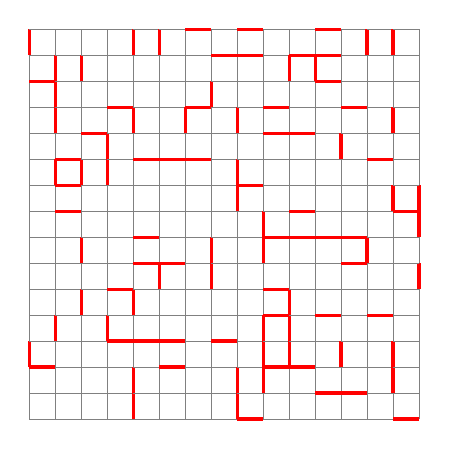
\begin{tikzpicture}
        \def\p{0.2}
        \foreach \x in {0,0.33,...,4.63} {
            \foreach \y in {0,0.33,...,4.63} {
                \pgfmathparse{rnd}
                \ifdim\pgfmathresult pt < \p pt\relax 
                    \draw[red, very thick] (\x, \y) -- (\x, \y + 0.33);
                \else
                    \draw[gray] (\x, \y) -- (\x, \y + 0.33);
                \fi 
                \pgfmathparse{rnd}
                \ifdim\pgfmathresult pt < \p pt\relax
                    \draw[red, very thick] (\x, \y) -- (\x + 0.33, \y);
                \else
                    \draw[gray] (\x, \y) -- (\x + 0.33, \y);
                \fi 
            }
            \pgfmathparse{rnd}
            \ifdim\pgfmathresult pt < \p pt\relax
                \draw[red, very thick] (\x, 4.95) -- (\x + 0.33, 4.95);
            \else
                \draw[gray] (\x, 4.95) -- (\x + 0.33, 4.95);
            \fi
            \pgfmathparse{rnd}
            \ifdim\pgfmathresult pt < \p pt\relax
                \draw[red, very thick] (4.95, \x) -- (4.95, \x + 0.33);
            \else
                \draw[gray] (4.95, \x) -- (4.95, \x + 0.33);
            \fi
        }
    \end{tikzpicture}
    \caption*{$p = 0.2$}
    \endminipage\hfill
    \minipage{0.32\textwidth}
    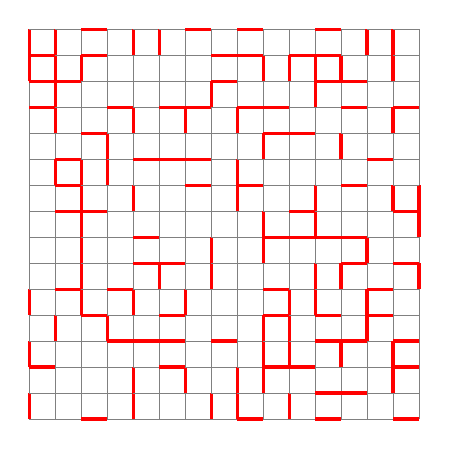
\begin{tikzpicture}
        \def\p{0.3}
        \foreach \x in {0,0.33,...,4.63} {
            \foreach \y in {0,0.33,...,4.63} {
                \pgfmathparse{rnd}
                \ifdim\pgfmathresult pt < \p pt\relax 
                    \draw[red, very thick] (\x, \y) -- (\x, \y + 0.33);
                \else
                    \draw[gray] (\x, \y) -- (\x, \y + 0.33);
                \fi 
                \pgfmathparse{rnd}
                \ifdim\pgfmathresult pt < \p pt\relax
                    \draw[red, very thick] (\x, \y) -- (\x + 0.33, \y);
                \else
                    \draw[gray] (\x, \y) -- (\x + 0.33, \y);
                \fi 
            }
            \pgfmathparse{rnd}
            \ifdim\pgfmathresult pt < \p pt\relax
                \draw[red, very thick] (\x, 4.95) -- (\x + 0.33, 4.95);
            \else
                \draw[gray] (\x, 4.95) -- (\x + 0.33, 4.95);
            \fi
            \pgfmathparse{rnd}
            \ifdim\pgfmathresult pt < \p pt\relax
                \draw[red, very thick] (4.95, \x) -- (4.95, \x + 0.33);
            \else
                \draw[gray] (4.95, \x) -- (4.95, \x + 0.33);
            \fi
        }
    \end{tikzpicture}
    \caption*{$p = 0.3$}
    \endminipage\hfill
    \minipage{0.32\textwidth}
    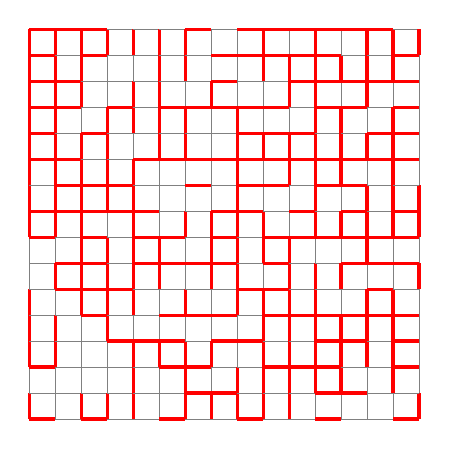
\begin{tikzpicture}
        \def\p{0.6}
        \foreach \x in {0,0.33,...,4.63} {
            \foreach \y in {0,0.33,...,4.63} {
                \pgfmathparse{rnd}
                \ifdim\pgfmathresult pt < \p pt\relax 
                    \draw[red, very thick] (\x, \y) -- (\x, \y + 0.33);
                \else
                    \draw[gray] (\x, \y) -- (\x, \y + 0.33);
                \fi 
                \pgfmathparse{rnd}
                \ifdim\pgfmathresult pt < \p pt\relax
                    \draw[red, very thick] (\x, \y) -- (\x + 0.33, \y);
                \else
                    \draw[gray] (\x, \y) -- (\x + 0.33, \y);
                \fi 
            }
            \pgfmathparse{rnd}
            \ifdim\pgfmathresult pt < \p pt\relax
                \draw[red, very thick] (\x, 4.95) -- (\x + 0.33, 4.95);
            \else
                \draw[gray] (\x, 4.95) -- (\x + 0.33, 4.95);
            \fi
            \pgfmathparse{rnd}
            \ifdim\pgfmathresult pt < \p pt\relax
                \draw[red, very thick] (4.95, \x) -- (4.95, \x + 0.33);
            \else
                \draw[gray] (4.95, \x) -- (4.95, \x + 0.33);
            \fi
        }
    \end{tikzpicture}
    \caption*{$p = 0.6$}
    \endminipage\hfill
\end{figure}

When $p = 0.2$ and $p = 0.3$, the clusters of red segments are isolated, whereas when $p = 0.6$, there exists such a cluster that connects the top and bottom sides. 

In addition, the size of a metal-oxide block is negligible when compared to the overall scale of a memresistor. It is therefore reasonable to think of an infinitely large grid. Since it is difficult to attain precise values of $p$, to allow more tolerance in the voltage supplied, we are more interested in knowing about the following: for what values of $p$ are we certain that no infinite clusters of conductive metal-oxide blocks exist? For what values of $p$ do we guarantee the existence of such an infinite cluster connecting the top and bottom electrodes?

What is described above forms the basis of percolation theory. Since its birth in 1957 due to Broadbent and Hammersley~\autocite*[693]{broadbent_hammersley_1957}, the problem has attracted pure mathematicians and scientists from myriad domains. Despite its simple formulation, the percolation model brings insight into the behaviour of many natural systems ranging from the flow of fluids through a disordered porous medium to the spread of forest fires and epidemics~\autocite[60]{gennes_2000}. Nevertheless, the first major mathematical result was not announced until only some twenty years later: in 1980, Kesten~\autocite*[41]{kesten_1980} completed Harris's 1960 work~\autocite*[13]{harris_1960} to ascertain the effect of the probability $p$ on the existence of infinite clusters on the square lattice, the model of memresistors used in this investigation. Nowadays, percolation theory is a growing field that interconnects mathematics, physics, and computer science. All three being my favourite disciplines, I happily delved into what appeared to me as an exotic crossover of probability and graph theory, both of which we have studied in class.

We start by stating a few definitions that allow a rigorous treatment of the subject. We then study the case where infinite clusters do not exist, and continue with the case where they do. We conclude with a discussion on the significance of the results and possible ways to extend the investigation.

\section{Definitions}\label{sec:prelims}
\begin{defn}\label{def:graph}
    A \textit{graph} $G = (V, E)$ models pairwise relations between \textit{vertices} in the set $V$. For the square lattice in question, the set $V$ is $\Z^2 = \{(x, y) \mid x, y \in \Z\}$. For $A(x_A, y_A), B(x_B, y_B) \in V$, we define that the unordered pair $\{A, B\}$ belongs to $E$ if and only if $\abs{x_A - x_B} + \abs{y_A - y_B} = 1$. We say $A$ and $B$ are neighbours if the \textit{edge} $\{A, B\} \in E$.
\end{defn}
\begin{ex*}\vspace{-0.01cm}
    The neighbours of the origin $(0, 0)$ are $(0, 1), (1, 0), (0, -1), (-1, 0)$.
    \begin{figure}[!hb]
    \centering
    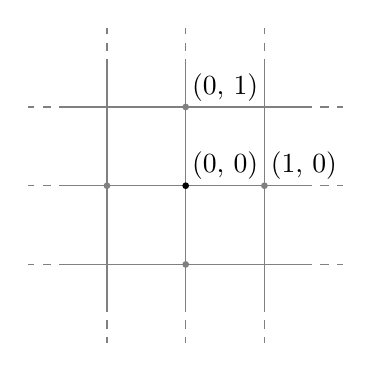
\begin{tikzpicture}
        \foreach \i in {-1, 0, 1} {
            \draw[gray] (-1.5, \i) -- (1.5, \i);
            \draw[gray] (\i, -1.5) -- (\i, 1.5);
            
            \draw[gray, dashed] (-1.5, \i) -- (-2.0, \i);
            \draw[gray, dashed] (\i, -1.5) -- (\i, -2.0);
            \draw[gray, dashed] (1.5, \i) -- (2.0, \i);
            \draw[gray, dashed] (\i, 1.5) -- (\i, 2.0);
        }
        \node at (0.5, 0.25) {(0, 0)};
        \node at (1.5, 0.25) {(1, 0)};
        \node at (0.5, 1.25) {(0, 1)};
        
        \filldraw (0, 0) circle (1pt);
        \filldraw[gray] (0, +1) circle (1pt);
        \filldraw[gray] (0, -1) circle (1pt);
        \filldraw[gray] (-1, 0) circle (1pt);
        \filldraw[gray] (+1, 0) circle (1pt);
    \end{tikzpicture}
    \caption{The origin (black) and its 4 neighbours (grey) on the square lattice}
    \label{fig:square_lattice}
\end{figure}
\end{ex*}

%We shall not get burdened with the measure-theoretic details about the probability space, but to avoid juggling with infinities in the model, some formal definitions are required.
%
%\begin{defn}\label{defn:outcome_and_event}
%We call a realisation an \textit{outcome}; e.g., the leftmost panel of \cref{fig:3_realisations} shows an outcome when $p = 0.2$. An \textit{event} is a set of zero or more outcomes, and depends on finitely many edges. We say an event \textit{occurs} if the outcome belongs to the event.
%\end{defn}
%
%\begin{ex}\label{ex:cluster_of_size_n}
%Let $n$ be a nonnegative integer. Recall that a \textit{self-avoiding path} of length $n$ is a sequence of vertices $v_1, v_2, \dots, v_{n + 1}$ that are all distinct.
%Let $C$ be the set of vertices that are connected to the origin $O$ via open edges (with $O \in C$). We define the event
%\[
%\{\abs{C} \geq n + 1\}
%= \{\text{there is a self-avoiding path of open edges of length } n \text{ from } O\}
%\]
%where $\abs{C}$ denotes the size of the cluster $C$.
%\begin{figure}[ht!]
    \centering
    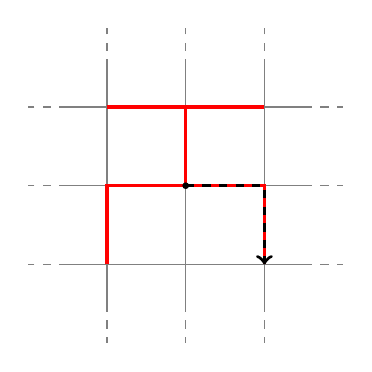
\begin{tikzpicture}
        \foreach \i in {-1, 0, 1} {
            \draw[gray] (-1.5, \i) -- (1.5, \i);
            \draw[gray] (\i, -1.5) -- (\i, 1.5);
            
            \draw[gray, dashed] (-1.5, \i) -- (-2.0, \i);
            \draw[gray, dashed] (\i, -1.5) -- (\i, -2.0);
            \draw[gray, dashed] (1.5, \i) -- (2.0, \i);
            \draw[gray, dashed] (\i, 1.5) -- (\i, 2.0);
        }
        
        \draw[red, very thick] (0, 0) -- (0, 1);
        \draw[red, very thick] (-1, 1) -- (1, 1);
        \draw[red, very thick] (-1, -1) -- (-1, 0) -- (0, 0);
        
        \draw[red, very thick] (0, 0) -- (1, 0) -- (1, -1);
        \draw[->, dashed, very thick] (0, 0) -- (1, 0) -- (1, -1);
        
        \filldraw (0, 0) circle (1pt);
        
    \end{tikzpicture}
    \caption{A self-avoiding path of length $2$ from $O$: the event $\abs{C} \geq 3$ occurs.}
    \label{fig:cluster_self_avoiding_path}
\end{figure}
%\end{ex}
%
\begin{defn}\label{def:event_prob}
Let $A$ be an \textit{event}. We use $\Pp(A)$ to denote the probability of $A$ occurring for a fixed value of the parameter $p$. With $B$ being another event, $\Pp(A)$ and $\Pp(B)$ satisfy:
\begin{itemize}
    \item $0 \leq \Pp(A) \leq 1$ --- in particular, $\Pp(\varnothing) = 0$;
    \item $\Pp(A \cup B) = \Pp(A) + \Pp(B) - \Pp(A \cap B)$;
    \item $A$ is the \textit{complement} of $B$ if and only if $\Pp(A) = 1 - \Pp(B)$;
    \item $A$ and $B$ are \textit{independent} if and only if $\Pp(A \cap B) = \Pp(A) \Pp(B)$.
\end{itemize}
\end{defn}

\begin{lem}[Monotonicity]\label{lem:event_subseteq}
If the occurrence of event $A$ implies the occurrence of event $B$, then $$\Pp(A) \leq \Pp(B).$$
\end{lem}
\begin{proof}
For any two events $A$ and $B$, we have
\begin{align*}
    \Pp(B) 
    &= \Pp(A \cup (B \setminus A))\\
    &= \Pp(A) + \Pp(B \setminus A) - \Pp(A \cap (B \setminus A))\\
    \therefore \Pp(B) &- \Pp(A) = \Pp(B \setminus A) - \Pp(A \cap (B \setminus A))
\end{align*}
\begin{figure}[h]
    \centering
    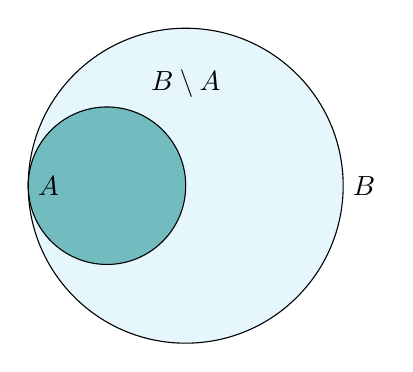
\begin{tikzpicture}
        \def\bigcircle{(1, 0) circle (2cm)}
        \def\smallcircle{(0, 0) circle (1cm)}
        \fill[cyan, fill opacity=0.1] \bigcircle;
        \fill[teal, fill opacity=0.5] \smallcircle;
        \draw \smallcircle;
        \draw \bigcircle;
        
        \node[right] at (-1, 0) {$A$};
        \node[right] at (3, 0) {$B$};
        \node[above] at (1, 1) {$B \setminus A$};
     \end{tikzpicture}
    \caption{Venn diagram of the event sets $A$ and $B$}
    \label{fig:venn}
\end{figure}


Here, $A$ and $B$ are two sets where, for all $\omega \in A$, we also have $\omega \in B$. Hence, $A \subseteq B$ as shown in \cref{fig:venn}. We then have $A \cap (B \setminus A) = \varnothing$, and as such $\Pp(A \cap (B \setminus A)) = 0$. Then, since $\Pp(B \setminus A) \geq 0$ by \cref{def:event_prob}, 
\begin{align*}
\Pp(B) - \Pp(A) &= \Pp(B \setminus A) - 0 \geq 0\\
\therefore \Pp(B) &\geq \Pp(A)
\end{align*}
as claimed.
\end{proof}

\begin{defn}
    Let $p \in [0, 1]$. For each edge $e \in E$, we declare $e$ to be \textit{open} with probability $p$ and \textit{closed} otherwise with probability $1 - p$, independently of the states of other edges. We call the resulting collection of open edges a \textit{percolation realisation}.
\end{defn}
\begin{ex*}
    \Cref{fig:cluster_self_avoiding_path} below shows a percolation realisation on a $3 \times 3$ subsection of the square lattice for $p = 0.5$. The open edges are coloured in red; the closed edges are in grey.
\end{ex*}

\begin{defn}\label{def:path}
    Let $n$ be a nonnegative integer. A \textit{path} of length $n$ is a sequence of vertices $v_0, v_1, \dots, v_{n}$ that are all distinct and connected --- $\forall i \in \{0, 1, \dots, n - 1\}, \{v_i ,v_{i + 1}\} \in E$. The path is \textit{open} if we have further that each edge $\{v_i, v_{i + 1}\}$ is open. In that case, we say $v_0$ is connected to $v_{n}$.
\end{defn}
\begin{ex*}\end{ex*}
\begin{figure}[ht!]
    \centering
    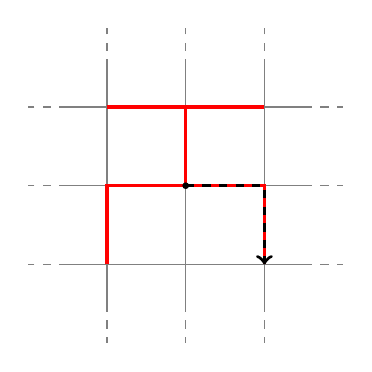
\begin{tikzpicture}
        \foreach \i in {-1, 0, 1} {
            \draw[gray] (-1.5, \i) -- (1.5, \i);
            \draw[gray] (\i, -1.5) -- (\i, 1.5);
            
            \draw[gray, dashed] (-1.5, \i) -- (-2.0, \i);
            \draw[gray, dashed] (\i, -1.5) -- (\i, -2.0);
            \draw[gray, dashed] (1.5, \i) -- (2.0, \i);
            \draw[gray, dashed] (\i, 1.5) -- (\i, 2.0);
        }
        
        \draw[red, very thick] (0, 0) -- (0, 1);
        \draw[red, very thick] (-1, 1) -- (1, 1);
        \draw[red, very thick] (-1, -1) -- (-1, 0) -- (0, 0);
        
        \draw[red, very thick] (0, 0) -- (1, 0) -- (1, -1);
        \draw[->, dashed, very thick] (0, 0) -- (1, 0) -- (1, -1);
        
        \filldraw (0, 0) circle (1pt);
        
    \end{tikzpicture}
    \caption{A self-avoiding path of length $2$ from $O$: the event $\abs{C} \geq 3$ occurs.}
    \label{fig:cluster_self_avoiding_path}
\end{figure}

\begin{defn}\label{def:cluster}
    The \textit{cluster centred at the origin} is the set of vertices that are connected to $O(0, 0)$. We denote this set by $C$. Note that $O \in C$.
\end{defn}
\begin{ex*}
    In \cref{fig:cluster_self_avoiding_path}, $C = \{(-1, -1), (-1, 0), (-1, 1), (0, 0), (0, 1), (1, -1), (1, 0), (1, 1)\}$.
\end{ex*}

\begin{defn}\label{def:inf_cluster}
    $\abs{C}$ denotes the number of vertices in $C$. We write $\abs{C} = \infty$ if $C$ is an \textit{infinite cluster}, i.e., when there are arbitrarily many vertices that are connected to $O(0, 0)$ via open paths. We use $\theta(p)$ to refer to $\Pp(\abs{C} = \infty)$, the probability that the cluster centred at the origin on the square lattice is an infinite cluster as a function of the parameter $p$.
\end{defn}

\begin{rem*}
    Every vertex on the square lattice $\Z^2$ plays the same role. As a consequence, although $\theta(p)$ concerns the cluster centred at the origin, it equally describes the probability of an infinite cluster centred at any other vertex. More specifically, $\theta(p) = 0$ means that there does not exist any infinite cluster, and $\theta(p) > 0$ means that there exists an infinite cluster somewhere on the square lattice.
\end{rem*}

\section{$\theta(p) = 0$}\label{sec:no_inf}
Clearly, when $p = 0$, there are no open edges at all; $C = \{(0, 0)\}$ and $\theta(p) = 0$ necessarily. To find other non-trivial solutions, we firstly need to find a relation involving $\theta(p)$.

\begin{defn}\label{def:set_paths}
    Let $n \in \N$. We use $\Omega_n$ to denote the set of paths (open or not) of length $n$ from $O(0, 0)$.
\end{defn}

It follows from \cref{def:inf_cluster} that if $\abs{C} = \infty$, then for any $n \in \N$, there exists an open path  of length $n$ starting from $O(0, 0)$; i.e., there exists a path $\gamma \in \Omega_n$ that is open. Mathematically, the event $\abs{C} = \infty$ implies the event $(\bigcup_{\gamma \in \Omega_n} \gamma \text{ is open})$. By \cref{lem:event_subseteq},
\begin{align}\label{eq:theta_p_higher_union}
    \theta(p) = \Pp(\abs{C} = \infty) \leq \Pp(\bigcup_{\gamma \in \Omega_n} \gamma \text{ is open}).
\end{align}
The union of events in the expression above does not help us with finding $p$. Nevertheless, we can make use of the following lemma.

\begin{lem}[Boole's inequality]\label{lem:union_bound}
$\Pp(A_1 \cup A_2 \cup \cdots \cup A_n) \leq \Pp(A_1) + \Pp(A_2) + \cdots + \Pp(A_n)$
\end{lem}
\begin{proof}[Proof]
We proceed by induction on $n$. Let $\mathcal{P}(n): \Pp(\bigcup_{i = 1}^n A_i) \leq \sum_{i = 1}^n \Pp(A_i)$ for  $n \in \N^*$.
\begin{description}
\item \textit{Base case. } We have $\Pp(A_1) \leq \Pp(A_1)$, and hence $\mathcal{P}(1)$ is true.
\item \textit{Inductive step. } Assume that $\mathcal{P}(k)$ is true for a certain $k \in \N^*$; show that $\mathcal{P}(k + 1)$ is true.
We use the associative property of the union operation:
\begin{align*}
    \Pp(\bigcup_{i = 1}^{k + 1} A_i) 
    &= \Pp(\bigcup_{i = 1}^{k} A_i \cup A_{k + 1})\\
    &= \Pp(\bigcup_{i = 1}^{k} A_i) + \Pp(A_{k + 1}) - \Pp(\bigcup_{i = 1}^{k} A_i \cap A_{k + 1})\\
    &\leq \sum_{i = 1}^k \Pp(A_i) + \Pp(A_{k + 1}) - \Pp(\bigcup_{i = 1}^{k} A_i \cap A_{k + 1})\\
\end{align*}
Since $\Pp(\bigcup_{i = 1}^{k} A_i \cap A_{k + 1}) \geq 0$, we can conclude that $\Pp(\bigcup_{i = 1}^{k + 1} A_i) \leq \sum_{i = 1}^{k + 1} \Pp(A_i)$.
\end{description}
By the principle of mathematical induction, $\mathcal{P}(n)$ is true for any $n \in \N^*$.
\end{proof}

We can deduce from \cref{eq:theta_p_higher_union} that
\begin{align}\label{eq:theta_p_higher_sum}
    \theta(p) \leq \Pp(\bigcup_{\gamma \in \Omega_n} \gamma \text{ is open}) \leq \sum_{\gamma \in \Omega_n} \Pp(\gamma \text{ is open}).
\end{align}

\begin{prop}\label{prop:path_open}
    For all path $\gamma \in \Omega_n$, $\Pp(\gamma \text{ is open}) = p^n$.
\end{prop}
\begin{proof}
    Let $\gamma \in \Omega_n$. The path $\gamma$ is of length $n$ and has $n$ edges. Since each edge is open with probability $p$ independently, the probability that all $n$ edges are open is equal to $p^n$.
\end{proof}

\begin{prop}\label{prop:omega_size}
    Let $\abs{\Omega_n}$ denote the number of paths of length $n$ from $O(0, 0)$. For $n \in \N$, we have $\abs{\Omega_n} \leq 4 \times 3^{n - 1}$.
\end{prop}
\begin{proof}
    Firstly, we prove that $\abs{\Omega_n} \leq 4 \times 3^{n - 1}$ holds for $n \in \N^*$ by induction.
    \begin{figure}[!h]
    \centering
    \caption{Enumeration of self-avoiding paths in $\Z^2$}
    \label{fig:nb_self_avoiding_path}
    \minipage{0.5\textwidth}
    \centering
    \begin{tikzpicture}
        \foreach \i in {-1, 0, 1} {
            \draw[gray] (-1.5, \i) -- (1.5, \i);
            \draw[gray] (\i, -1.5) -- (\i, 1.5);
            \draw[gray, dashed] (-1.5, \i) -- (-2.0, \i);
            \draw[gray, dashed] (\i, -1.5) -- (\i, -2.0);
            \draw[gray, dashed] (1.5, \i) -- (2.0, \i);
            \draw[gray, dashed] (\i, 1.5) -- (\i, 2.0);
        }
        
        \filldraw (0, 0) circle (1pt);
        \draw[->, thick] (0, 0) -- (1, 0);
        \draw[->, thick] (0, 0) -- (0, 1);
        \draw[->, thick] (0, 0) -- (-1, 0);
        \draw[->, thick] (0, 0) -- (0, -1);
    \end{tikzpicture}
    \caption*{$4$ choices for the first step}
    \endminipage\hfill
    % --
    \minipage{0.5\textwidth}
    \centering
    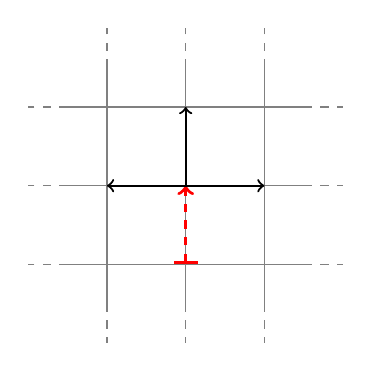
\begin{tikzpicture}
        \foreach \i in {-1, 0, 1} {
            \draw[gray] (-1.5, \i) -- (1.5, \i);
            \draw[gray] (\i, -1.5) -- (\i, 1.5);
            
            \draw[gray, dashed] (-1.5, \i) -- (-2.0, \i);
            \draw[gray, dashed] (\i, -1.5) -- (\i, -2.0);
            \draw[gray, dashed] (1.5, \i) -- (2.0, \i);
            \draw[gray, dashed] (\i, 1.5) -- (\i, 2.0);
        }
        
        \draw[|->, red, dashed, very thick] (0, -1) -- (0, 0);
        \draw[->, thick] (0, 0) -- (1, 0);
        \draw[->, thick] (0, 0) -- (0, 1);
        \draw[->, thick] (0, 0) -- (-1, 0);
    \end{tikzpicture}
    \caption*{$3$ choices for any step that follows}
    \endminipage
\end{figure}
    \begin{description}
        \item \textit{Base case. }
As shown in \cref{fig:square_lattice}, $O(0, 0)$ has $4$ neighbours. A path of length $1$ from $O$ starts at $O$ at finishes at a neighbour of $O$. As such, there are $4$ paths of length $1$ from $O$ as illustrated in \cref{fig:nb_self_avoiding_path}; i.e., $\abs{\Omega_1} = 4$. Indeed, $4 \leq 4 \times 3^{1 - 1}$ as claimed.
        \item \textit{Inductive step. }
Let $k \in \N^*$. Given that $\abs{\Omega_k} \leq 4 \times 3^{k - 1}$, we wish to prove that $\abs{\Omega_{k + 1}} \leq 4 \times 3^k$.

Let $\gamma$ be a path from $\Omega_k$. By the definition of the set $\Omega_k$, $\gamma = O, \dots, v_{k - 1}, v_k$. Although $v_k$ has $4$ neighbours, the path can not pass by $v_{k - 1}$ again, so we can only continue the path in \textbf{at most} $3$ directions (see \cref{fig:nb_self_avoiding_path}). There are already at most $4 \times 3^{k - 1}$ paths of length $k$ by the induction hypothesis, and from each of these paths, we can find at most $3$ paths of length $k + 1$. As such, $\abs{\Omega_{k + 1}} \leq 3 \times (4 \times 3^{k - 1}) = 4 \times 3^{k}$.
\end{description}
By the principle of mathematical induction, $\abs{\Omega_n} \leq 4 \times 3^{n - 1}, \forall n \in \N^*$. Additionally, $\Omega_0 = \{O\}$, and $\abs{\Omega_0} = 1 \leq 4 \times 3^{0 - 1}$, so the proposition extends to $n \in \N$.
\end{proof}

It follows from \cref{eq:theta_p_higher_sum} that
\begin{align}\label{eq:theta_leq_0}
    \theta(p) &\leq \sum_{\gamma \in \Omega_n} p^n\nonumber\\
    &\leq (4 \times 3^{n - 1}) \cdot p^n\nonumber\\
    &= \frac{4}{3} (3p)^n
\end{align}

With $3p < 1$ (i.e., $p < \frac{1}{3}$), when $n$ tends toward infinity, $\frac{4}{3}(3p)^n$ tends toward $0$. From \cref{eq:theta_leq_0}, when $n \to \infty$, we have $\theta(p) \leq 0$. Yet $\theta(p) \geq 0$ since the probability of an event is non-negative, so $\theta(p) = 0$ when $p < \frac{1}{3}$. Therefore, $p < \frac{1}{3}$ is a sufficient condition for the insulation of a memresistor, i.e., that there exists no infinite cluster on the square lattice.


\section{$\theta(p) > 0$}\label{sec:yes_inf}
It is obvious that when $p = 1$, all edges are open and there exists an infinite cluster that contains all the vertices in the square lattice; i.e., $\theta(1) = 1$. Of course, we are interested in finding other solutions for $\theta(p) > 0$.

Compared to the case where $\theta(p) = 0$, solving for $\theta(p) > 0$ was a much more difficult task. My research pointed me to the \textit{Peierls argument}, named after the British physicist who proved a phase transition~\autocite*[477]{peierls_1936} --- the change of macroscopic behaviour as the parameter varies, e.g., the appearance of an infinite cluster --- for the Ising model, another probabilistic model in statistical physics that explains the phenomenon of ferromagnetism. Instead of trying to directly find a lower bound on $\theta(p)$, we establish an upper bound on $1 - \theta(p)$ using the concept of a dual graph.

\begin{defn}\label{defn:dual_graph}
A \textit{planar graph} is a graph that can be drawn on the plane without its edges crossing. For instance, the square lattice is a planar graph. Given a planar graph $G$, we define its \textit{dual graph} $G^*$ in such a way that:
\begin{itemize}
    \item $G^*$ has a vertex for each face delimited by edges of $G$;
    \item an edge connects two vertices of $G^*$ if the corresponding faces are separated by an edge of $G$.
\end{itemize}
\end{defn}

\begin{ex*}
    We construct $\Zdual$, the dual graph of the square lattice $\Z^2$, by a vector transformation of $(\frac{1}{2}, \frac{1}{2})$ of the vertices: 
    \begin{figure}[h!]
    \centering
    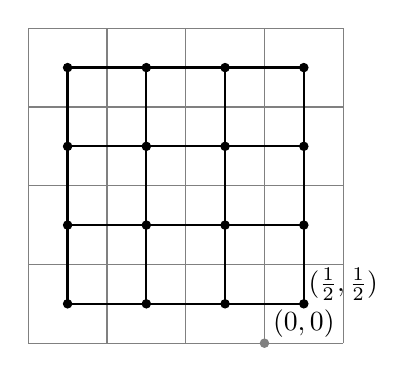
\begin{tikzpicture}
        % Z^2
        \foreach \x in {0, 1, ..., 4} {
            \draw[gray] (0, \x) -- (4, \x);
            \draw[gray] (\x, 0) -- (\x, 4);
        }
        
        % Z^2 dual
        \foreach \i in {0.5, 1.5, ..., 3.5} {
            \draw[black, thick] (0.5, \i) -- (3.5, \i);
            \draw[black, thick] (\i, 0.5) -- (\i, 3.5);
            \foreach \j in {0.5, 1.5, ..., 3.5} {
                \filldraw[black] (\i, \j) circle (1.5pt);
            }
        }
        
        \filldraw[gray] (3.0, 0.0) circle (1.5pt); 
        
        \node at (3.5, 0.25) {$(0, 0)$};
        \node at (4.0, 0.75) {$(\frac{1}{2}, \frac{1}{2})$};
                
    \end{tikzpicture}
    \caption{A $5 \times 5$ section of the square lattice and its dual}
    \label{fig:dual}
\end{figure}
    
    We notice that each edge of $\Z^2$ corresponds uniquely to an edge of $\Zdual$, namely the edge in the dual graph that it crosses. Let $(x, y) \in \Z^2$. The vertical edge $\{(x, y), (x, y + 1)\}$ corresponds to the horizontal edge $\{(x - \frac{1}{2}, y + \frac{1}{2}), (x + \frac{1}{2}, y + \frac{1}{2})\}$ in the dual graph; the edge $\{(x, y), (x + 1, y)\}$ corresponds to $\{(x + \frac{1}{2}, y - \frac{1}{2}), (x + \frac{1}{2}, y + \frac{1}{2})\}$ in the dual graph. 
\end{ex*}

\begin{defn}\label{def:dual_percolation}
    We define the \textit{dual} of a percolation realisation on $\Z^2$ as follows. Let $e^*$ be an edge on the dual graph $\Zdual$ that crosses the edge $e$ on the square lattice $\Z^2$. The edge $e^*$ is \textit{open} if and only if $e$ is \textit{closed}; in that case, we say $e^*$ `blocks' $e$.
\end{defn}

\begin{rem*}
    The event that $e^*$ is open is the complement of the event that $e$ is open. Since the latter occurs with a probability of $p$, each edge in the dual graph $\Zdual$ is open with a probability of $1 - p$.
\end{rem*}

\begin{ex*}
    \Cref{fig:square_lattice_dual} shows the dual of a percolation realisation. The intersection points of the grey grid are the vertices in $\Z^2$; the black dots are the vertices in $\Zdual$. The red edges represent the open edges on the square lattice $\Z^2$; the blue edges represent the open edges on the dual lattice $\Zdual$.
    \begin{figure}[h!]
    \centering
    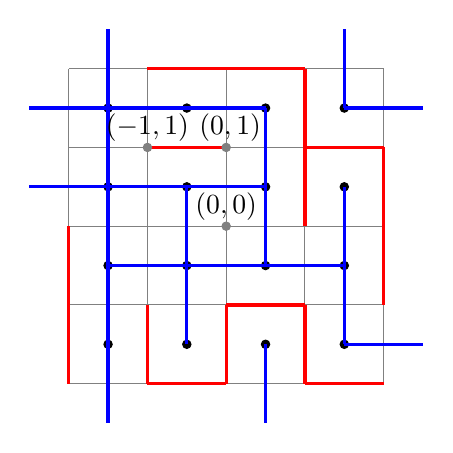
\begin{tikzpicture}
        % Grid
        \foreach \x in {0, 1, ..., 4} {
            \draw[gray] (0, \x) -- (4, \x);
            \draw[gray] (\x, 0) -- (\x, 4);
        }
        
        
        \foreach \i in {0.5, 1.5, ..., 3.5} {
            \foreach \j in {0.5, 1.5, ..., 3.5} {
                \filldraw[black] (\i, \j) circle (1.5pt);
            }
        }
        
        % Percolation
        %% |
        \draw[red, very thick] (0, 2) -- (0, 0);
        \draw[red, very thick] (1, 1) -- (1, 0);
        \draw[red, very thick] (2, 1) -- (2, 0);
        \draw[red, very thick] (3, 4) -- (3, 2); 
        \draw[red, very thick] (3, 1) -- (3, 0);
        \draw[red, very thick] (4, 3) -- (4, 1);
        %% -
        \draw[red, very thick] (1, 4) -- (3, 4);
        \draw[red, very thick] (1, 3) -- (2, 3);
        \draw[red, very thick] (3, 3) -- (4, 3);
        \draw[red, very thick] (2, 1) -- (3, 1);
        \draw[red, very thick] (1, 0) -- (2, 0);
        \draw[red, very thick] (3, 0) -- (4, 0);
        
        % Dual percolation
        %% -
        \draw[blue, very thick] (-0.5, 3.5) -- (2.5, 3.5);
        \draw[blue, very thick] (3.5, 3.5) -- (4.5, 3.5);
        \draw[blue, very thick] (-0.5, 2.5) -- (2.5, 2.5);
        \draw[blue, very thick] (0.5, 1.5) -- (3.5, 1.5);
        \draw[blue, very thick] (3.5, 0.5) -- (4.5, 0.5);
        %% |
        \draw[blue, very thick] (0.5, 4.5) -- (0.5, -0.5);
        \draw[blue, very thick] (1.5, 2.5) -- (1.5, 0.5);
        \draw[blue, very thick] (2.5, 3.5) -- (2.5, 1.5);
        \draw[blue, very thick] (2.5, 0.5) -- (2.5, -0.5);
        \draw[blue, very thick] (3.5, 4.5) -- (3.5, 3.5);
        \draw[blue, very thick] (3.5, 2.5) -- (3.5, 0.5);
        
        \node at (2, 2.25) {$(0, 0)$};
        \filldraw[gray] (2, 2) circle (1.5pt);
        
        \node at (1, 3.25) {$(-1, 1)$};
        \filldraw[gray] (1, 3) circle (1.5pt);
        \node at (2.05, 3.25) {$(0, 1)$};
        \filldraw[gray] (2, 3) circle (1.5pt);
    \end{tikzpicture}
    \caption{A percolation realisation on a $5 \times 5$ section of the square lattice and its dual}
    \label{fig:square_lattice_dual}
\end{figure}
\end{ex*}

\begin{defn}\label{def:cycle}
    Let $n \in \N$. A \textit{cycle} of length $n$ is a sequence of vertices $v_0, v_1, \dots, v_{n - 1}, v_0$ such that $v_0, v_1, \dots, v_{n - 1}$ are all distinct and connected; in addition, $v_0, v_{n - 1}$ are connected.
\end{defn}
\begin{ex}\label{ex:cycle}
    $\{(\frac{1}{2}, \frac{1}{2}), (\frac{1}{2}, -\frac{1}{2}), (-\frac{1}{2}, -\frac{1}{2}), (-\frac{1}{2}, \frac{1}{2}), (\frac{1}{2}, \frac{1}{2})\}$ is a cycle of length $4$ on $\Zdual$.
\end{ex}

We say a cluster is \textit{finite} when it only contains finitely many vertices. Notice how, in \cref{fig:square_lattice_dual}, the finite clusters on the square lattice in red (e.g., $\{(0, 0)\}$ and $\{(-1, 1), (0, 1)\}$) are surrounded by a cycle of open edges in blue on the dual lattice. Similarly, we can describe the event that the cluster centred at the origin is finite, i.e., $\abs{C} < \infty$, using the existence of a cycle of open edges on the dual lattice $\Zdual$.

\begin{prop}\label{prop:cycle_finite}
    $\abs{C} < \infty$ if and only if there exists $n \in \N$ such that there is a cycle of open edges on the dual lattice $\Zdual$ surrounding $O(0, 0)$ that passes through the point $(n + \frac{1}{2}, \frac{1}{2})$.
\end{prop}
\begin{proof}
    By \cref{def:dual_percolation}, the cycle of open edges on $\Zdual$ means that all edges on $\Z^2$ connecting the vertices inside and the vertices outside of the cycle are closed. The cluster centred at the origin then contains only finitely many vertices, namely a subset of those that are enclosed within the cycle.
    
    Conversely, if the cluster centred at the origin is finite, then there exist open edges on $\Zdual$ that `block' the edges connecting vertices in the cluster and vertices outside the cluster. From these open edges on $\Zdual$ that contour the cluster, it is possible to find a cycle that surrounds $O(0, 0)$~\autocite[14--15]{grimmett_1999}. The `right side' of the cycle then must contain an edge that intersects the line $y = 0$ at a positive $x$-coordinate in $\Zdual$. Specifically, there exists an integer $n \in \N$ such that the edge $\{(n + \frac{1}{2}, \frac{1}{2}), (n + \frac{1}{2}, -\frac{1}{2})\}$ belongs to the cycle. As an illustration, in \cref{fig:square_lattice_dual}, one cycle of open edges surrounding the origin is the cycle of length $4$ in \cref{ex:cycle}, which contains $(\frac{1}{2}, \frac{1}{2})$.
\end{proof}

\begin{prop}\label{prop:cylce_implies_path}
Let $n \in \N$. If there exists a cycle in $\Zdual$ surrounding $O(0, 0)$ that passes by $(n + \frac{1}{2}, \frac{1}{2})$, then there exists a path of length $2n + 3$ in $\Zdual$ starting from $(n + \frac{1}{2}, \frac{1}{2})$.
\end{prop}
\begin{proof}
    The shortest cycle surrounding $O(0, 0)$ that passes by the point $(n + \frac{1}{2}, \frac{1}{2})$ is a rectangle whose vertices are $(n + \frac{1}{2}, \frac{1}{2}), (n + \frac{1}{2}, -\frac{1}{2}), (-\frac{1}{2}, -\frac{1}{2}), (-\frac{1}{2}, \frac{1}{2})$ --- see \cref{fig:shortest_cycle_dual}.
    \begin{figure}[!h]
    \centering
    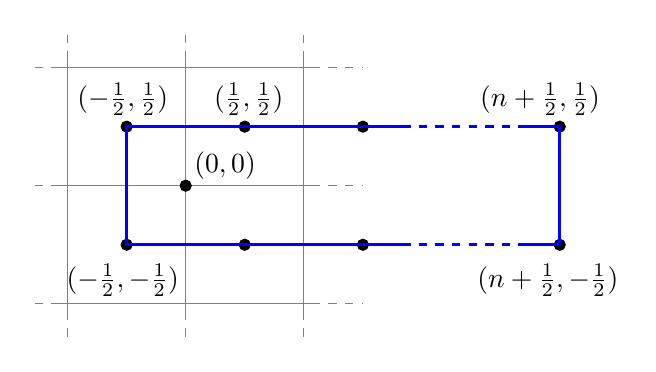
\begin{tikzpicture}
        \draw[gray] (-1.6, 1.5) -- (1.6, 1.5);
        \draw[gray] (-1.6, 0.0) -- (1.6, 0.0);
        \draw[gray] (-1.6, -1.5) -- (1.6, -1.5);
        
        \draw[gray] (-1.5, 1.6) -- (-1.5, -1.6);
        \draw[gray] (0.0, 1.6) -- (0.0, -1.6);
        \draw[gray] (1.5, 1.6) -- (1.5, -1.6);
        
        \draw[gray, dashed] (-1.5, -1.6) -- (-1.5, -2.0);
        \draw[gray, dashed] (0, -1.6) -- (0, -2.0);
        \draw[gray, dashed] (1.5, -1.6) -- (1.5, -2.0);
        
        \draw[gray, dashed] (-1.5, 1.6) -- (-1.5, 2.0);
        \draw[gray, dashed] (0, 1.6) -- (0, 2.0);
        \draw[gray, dashed] (1.5, 1.6) -- (1.5, 2.0);
        
        \draw[gray, dashed] (-1.6, 1.5) -- (-2.0, 1.5);
        \draw[gray, dashed] (-1.6, 0.0) -- (-2.0, 0.0);
        \draw[gray, dashed] (-1.6, -1.5) -- (-2.0, -1.5);
        
        \draw[gray, dashed] (1.6, 1.5) -- (2.25, 1.5);
        \draw[gray, dashed] (1.6, 0.0) -- (2.25, 0.0);
        \draw[gray, dashed] (1.6, -1.5) -- (2.25, -1.5);
        
        % Origin
        \node at (0.5, 0.25) {$(0, 0)$};
        \filldraw (0, 0) circle (2.0pt);
        
        % Dual
        \filldraw[black] (0.75, 0.75) circle (2pt);
        \filldraw[black] (0.75, -0.75) circle (2pt);
        \filldraw[black] (-0.75, 0.75) circle (2pt);
        \filldraw[black] (-0.75, -0.75) circle (2pt);
        
        \filldraw[black] (2.25, 0.75) circle(2pt);
        \filldraw[black] (2.25, -0.75) circle(2pt);
        
        \filldraw[black] (4.75, 0.75) circle(2pt);
        \filldraw[black] (4.75, -0.75) circle(2pt);
        
        \node at (0.8, 1.10) {$(\frac{1}{2}, \frac{1}{2})$};
        \node at (-0.8, 1.10) {$(-\frac{1}{2}, \frac{1}{2})$};
        \node at (-0.8, -1.20) {$(-\frac{1}{2}, -\frac{1}{2})$};
        \node at (4.5, 1.10) {$(n + \frac{1}{2}, \frac{1}{2})$};
        \node at (4.6, -1.20) {$(n + \frac{1}{2}, -\frac{1}{2})$};
        
        % Cycle
        \draw[blue, very thick] (4.25, -0.75) -- (4.75, -0.75) -- (4.75, 0.75) -- (4.25, 0.75);
        \draw[blue, very thick] (2.75, -0.75) -- (-0.75, -0.75) -- (-0.75, 0.75) -- (2.75, 0.75);
        \draw[blue, very thick, dashed] (2.75, -0.75) -- (4.25, -0.75);
        \draw[blue, very thick, dashed] (2.75, 0.75) -- (4.25, 0.75);
    \end{tikzpicture}
    \caption{The shortest cycle in $(\Z^2)^*$ passing by $(n + \frac{1}{2}, \frac{1}{2})$ and surrounding $O$}
    \label{fig:shortest_cycle_dual}
\end{figure}
    
    This cycle is of length \[2 \times \left( \frac{1}{2} - (-\frac{1}{2})\right) + 2 \times \left((n + \frac{1}{2}) - (-\frac{1}{2})\right) = 2n + 4.\]
    By \cref{def:cycle}, this cycle is a sequence of vertices $v_0, v_1, \dots, v_{2n + 3}, v_{0}$ where $v_0 = (n + \frac{1}{2}, \frac{1}{2})$, and the vertices $v_0, v_1, \dots, v_{2n + 3}$ are all distinct and connected. Hence, the sequence of vertices $v_0, v_1, \dots, v_{2n + 3}$ forms a path of length $2n + 3$ by \cref{def:path}. 
    
All other cycles surrounding $(0, 0)$ passing by $(n + \frac{1}{2}, \frac{1}{2})$ zigzag through other points and have a length that is greater than $2n + 4$. However, we can find still a sequence of $2n + 3$ vertices $v_0, v_1, \dots, v_{2n + 3}$ from the cycle to obtain a path of length $2n + 3$ starting from $(n + \frac{1}{2}, \frac{1}{2})$.
\end{proof}

We can now find an upper bound on the probability that the cluster centred at the origin is finite using what is historically known as the Peierls argument.

\begin{align}
    \Pp(\abs{C} < \infty)
    &= \Pp\left(\bigcup_{n \in \N} \exists\,\text{cycle surrounding the origin passing by } (n + \frac{1}{2}, \frac{1}{2})\right)\label{eq:union_exists_cycle}\\
    &\leq \sum_{n \in \N} \Pp\left(\exists\,\text{cycle surrounding the origin passing by } (n + \frac{1}{2}, \frac{1}{2})\right)\label{eq:sum_exists_cycle}\\
    & \leq \sum_{n \in \N} \Pp\left(\exists\,\text{path of length } 2n + 3 \text{ passing by }(n + \frac{1}{2}, \frac{1}{2})\right)\label{eq:sum_exists_path}\\
    &\leq \sum_{n \in \N} \Pp(\bigcup_{\gamma \in \Omega_{2n + 3}} \text{the path } \gamma \text{ is open})\label{eq:sum_union_exists_path}\\
    &\leq \sum_{n \in \N} \sum_{\gamma \in \Omega_{2n + 3}} \Pp(\text{the path } \gamma \text{ is open})\label{eq:sum_sum_path_open}\\
    &\leq \sum_{n \in \N} (4 \cdot 3^{2n + 2}) (1 - p)^{2n + 3}\label{eq:sum_path_open}
\end{align}

\Cref{eq:union_exists_cycle} is a direct consequence of \cref{prop:cycle_finite}.

\Cref{eq:sum_exists_cycle} uses \cref{lem:union_bound} to decompose the probability of the union of events.

\Cref{eq:sum_exists_path} applies \cref{lem:event_subseteq} to the implication in \cref{prop:cylce_implies_path}.

Notice that the upper bound on $\abs{\Omega_n}$ given in \cref{prop:omega_size} is equally valid regardless where all paths in $\Omega_n$ start, whether it is $O(0, 0)$ or $(n + \frac{1}{2}, \frac{1}{2})$. We then arrive at \cref{eq:sum_union_exists_path}.

\Cref{eq:sum_sum_path_open,eq:sum_path_open} use the same reasoning from \cref{sec:no_inf} when we studied the case of $\theta(p) = 0$. The only difference is that, on the dual lattice $\Zdual$, the parameter becomes $1 - p$. Therefore, we adapt \cref{prop:path_open} to say that, for $n \in \N$, a path on the dual lattice of length $n$ is open with a probability of $(1 - p)^n$.

Before concluding the case of $\theta(p) > 0$, we need to show that the notions $\Pp(\bigcup_{n \in \N} A_n)$ and $\sum_{n \in \N} \Pp(A_n)$ used above are well defined, where $A_n$ denotes an arbitrary event. Let $N \in \N$. The range $n \in \N$ corresponds to $n \in \{0, 1, \dots, N\}$ when $N$ tends to infinity. It is evident that $\bigcup_{n \in \{0, 1, \dots, N\}} A_n$ is non-decreasing over $\N$: $\bigcup_{n \in \{0, 1, \dots, N\}} A_n$ implies $\bigcup_{n \in \{0, 1, \dots, N + 1\}} A_n$, and hence $\Pp(\bigcup_{n \in \{0, 1, \dots, N\}} A_n) \leq \Pp(\bigcup_{n \in \{0, 1, \dots, N + 1\}} A_n)$ by \cref{lem:event_subseteq}. Therefore, $\lim_{N \to \infty} \Pp(\bigcup_{n \in \{0, 1, \dots, N\}} A_n)$, albeit perhaps not finite, exists. Similarly, since $\Pp(A_n) \geq 0$, $\sum_{n \in \{0, 1, \dots, N\}} \Pp(A_n)$ is non-decreasing and $\lim_{N \to \infty} \sum_{n \in \{0, 1, \dots, N\}}\Pp(A_n)$ exists.

We continue by considering the sum from \cref{eq:sum_path_open}
\begin{align*}
    &\phantom{=} \sum_{n = 0}^N (4 \cdot 3^{2n + 2}) (1 - p)^{2n + 3}\\
    &= 4 \cdot 3^2 (1 - p)^3 \sum_{n = 0}^N \left(3 (1 - p)\right)^{2n}\\
    &= 36 (1 - p)^3 \sum_{n = 0}^N \left(9 (1 - p)^2\right)^n.
\end{align*}
As $N$ tends to infinity, the geometric series only converges when $\abs{9 (1 - p)^2} < 1$, i.e., when $-\frac{1}{3} < (1 - p) < \frac{1}{3}$. Since we specified that $p \in \left[0, 1\right]$, when $p > \frac{2}{3}$, the limit evaluates to
$
    \frac{36 (1 - p)^3}{1 - 9 (1 - p)^2}.
$

\begin{figure}[H]
    \centering
    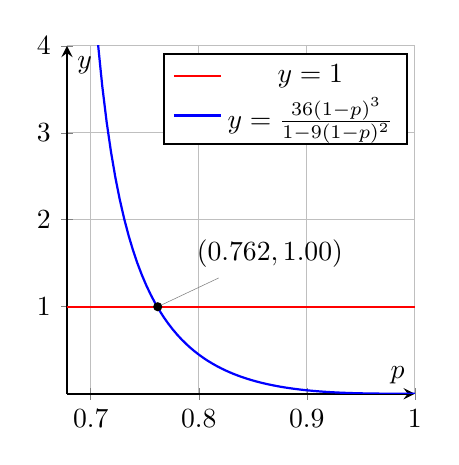
\begin{tikzpicture}
    \begin{axis}
    [xlabel={$p$}, 
     ylabel={$y$},
     axis lines=middle,
     grid,
     thick,
     domain=0.678:1,
     width=6cm,
     height=6cm,
     samples=80,
     ymin=0,
     ymax=4,
     %legend pos=outer north east
    ]
    \addplot+[no marks, red] {1};
    \addlegendentry{$y = 1$}
    \addplot+[no marks, blue] {(36 * (1-x)^3) / (1 - 9*(1-x)^2)};
    \addlegendentry{$y = \frac{36(1-p)^3}{1 - 9(1 - p)^2}$}
    \node[circle, fill=black, scale=0.35, pin=45:{$(0.762, 1.00)$}] at (axis cs:0.762, 1.0) {};
    \end{axis}
    \end{tikzpicture}
    \caption{The upper bound for $\P(\abs{C} < \infty)$}
    \label{fig:pc_upper_bound_plot}
\end{figure}

As shown in \cref{fig:pc_upper_bound_plot} opposite, graphically we can determine that for $p > 0.762$ approx., \[\Pp(\abs{C} < \infty) \leq \frac{36(1 - p)^3}{1 - 9(1 - p)^2} < 1.\]

Note that the event $\abs{C} < \infty$ is the complement of the event $\abs{C} = \infty$, and hence
\[
    \Pp(\abs{C} < \infty) = 1 - \Pp(\abs{C} = \infty) = 1 - \theta(p).
\]

We can now conclude that
\begin{align*}
    1 - \theta(p) &< 1\\
    \iff \theta(p) &> 0
\end{align*}
when $p > 0.762$ approximately.

%%\section{Percolation on the Cubic Lattice}
%%\subsection{The Cubic Lattice}
%%We can define the \textit{(simple) cubic lattice} $\Z^3$ in a similar fashion to the square lattice $\Z^2$: all the points that have integer coordinates $(x, y, z)$ constitute the set of vertices, and all the edges that connect two neighbouring points $A$ and $B$ on the cubic lattice, i.e., $\abs{A_x - B_x} + \abs{A_y - B_y} + \abs{A_z - B_z} = 1$, compose the set of edges. We use the same definition of the event $\{\abs{C} = \infty\}$ in terms of the existence of an arbitrarily long self-avoiding path.
%%
%%As with $\Z^2$, our interest lies in computing the value of the critical probability $p_c$ for $\Z^3$. We shall see how our work on the square lattice case will help us with proving a similar result on the cubic lattice, which in addition is closer to reality for modelling purposes.
%%
%%\subsection{The Critical Value}
%%\begin{thm}\label{thm:pc_on_Z3}
%%For Bernoulli bond percolation on $\Z^3$, we have $\dfrac{1}{5} \leq p_c \leq \dfrac{1}{2}$.
%%\end{thm}
%%\begin{proof}
%%Firstly, we use the reasoning from \cref{subsec:no_inf_cluster} to prove that $p_c > \frac{1}{5}$. For nonnegative integer $n$, let $\Omega_n$ denote the set of self-avoiding paths of length $n$ starting from the origin.
%%
%%\begin{figure}[!ht]
    \centering
    \caption{Enumeration of self-avoiding paths in $\Z^3$}
    \label{fig:z3_paths}
    \minipage{0.5\textwidth}
    \centering
    \begin{tikzpicture}
        \filldraw (0, 0) circle (1.5pt);
        \draw[->, thick] (0, 0) -- (2, 0);
        \draw[->, thick] (0, 0) -- (0, 2);
        \draw[->, thick] (0, 0) -- (-2, 0);
        \draw[->, thick] (0, 0) -- (0, -2);
        \draw[->, thick] (0, 0) -- (-1, -1);
        \draw[->, thick] (0, 0) -- (1, 1);
    \end{tikzpicture}
    \caption*{$6$ choices for the first step}
    \endminipage\hfill
    % --
    \minipage{0.5\textwidth}
    \centering
    \begin{tikzpicture}
        \draw[|->, very thick, red, dashed] (0, -2) -- (0, 0);
        
        \draw[->, thick] (0, 0) -- (2, 0);
        \draw[->, thick] (0, 0) -- (0, 2);
        \draw[->, thick] (0, 0) -- (-2, 0);
        \draw[->, thick] (0, 0) -- (-1, -1);
        \draw[->, thick] (0, 0) -- (1, 1);
    \end{tikzpicture}
    \caption*{$5$ choices for any step that follows}
    \endminipage
\end{figure}
%%
%%As shown in \cref{fig:z3_paths} above, there are at most $6 \cdot 5^{n - 1}$ paths in $\Omega_n$. Furthermore, for any path in $\Omega_n$, the probability that all its $n$ edges are open equals $p^n$.
%%
%%\begin{align*}
%%    \theta(p) 
%%    &= \lim_{n \to \infty} \Pp(\bigcup_{\gamma \in \Omega_n} \text{all the } n \text{ edges of } \gamma \text{ are open})\\
%%    &\leq \lim_{n \to \infty} \sum_{\gamma \in \Omega_n} p^n\\
%%    &\leq \lim_{n \to \infty} \left(6 \cdot 5^{n - 1}\right) p^n\\
%%    &= \lim_{n \to \infty} \frac{6}{5} (5 p)^{n}
%%\end{align*}
%%
%%The limit tends to 0 if $\abs{5p} < 1$. As such, if $p < \frac{1}{5}$, then $\theta(p) = 0$. Then, by the definition of $p_c$, we can deduce that $p_c \geq \frac{1}{5}$.
%%
%%Next, to show that $p_c \leq \frac{1}{2}$, one might be attempted to invoke the dual graph argument from \cref{subsec:inf_cluster}. Let us take a moment to consider what the dual graph of the cubic lattice would look like. Call to mind that we place a vertex for each face of $\Z^3$, and an edge for each edge of $\Z^3$ separating two faces.
%%
%%\begin{figure}[!h]
    \centering
    \centering
    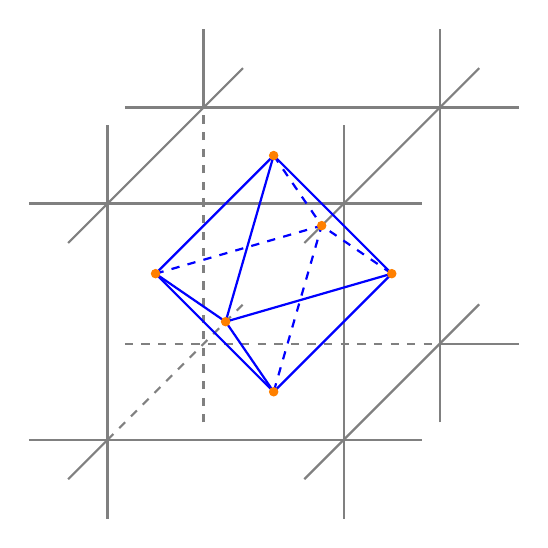
\begin{tikzpicture}
        % ---Z^3
        \draw[thick, gray] (-1, 0) -- (4, 0);
        \draw[thick, gray] (0, -1) -- (0, 4);
        \draw[thick, gray] (3, -1) -- (3, 4);
        \draw[thick, gray] (-1, 3) -- (4, 3);
        
        \draw[thick, gray, dashed] (0, 0) -- (1.72, 1.72);
        \draw[thick, gray] (-0.5, -0.5) -- (0, 0);
        \draw[thick, gray] (2.5, -0.5) -- (4.72, 1.72);
        \draw[thick, gray] (-0.5, 2.5) -- (1.72, 4.72);
        \draw[thick, gray] (2.5, 2.5) -- (4.72, 4.72);
        
        \draw[thick, gray, dashed] (1.22, 0.22) -- (1.22, 4.22);
        \draw[thick, gray] (1.22, 4.22) -- (1.22, 5.22);
        \draw[thick, gray, dashed] (0.22, 1.22) -- (4.22, 1.22);
        \draw[thick, gray] (4.22, 1.22) -- (5.22, 1.22);
        \draw[thick, gray] (4.22, 0.22) -- (4.22, 5.22);
        \draw[thick, gray] (0.22, 4.22) -- (5.22, 4.22);
        % \draw[thick] (0, 0) -- (3, 0);
        % \draw[thick] (0, 0) -- (0, 3);
        % \draw[thick] (3, 0) -- (3, 3);
        % \draw[thick] (0, 3) -- (3, 3);
        
        % \draw[thick, dashed] (0, 0) -- (1.22, 1.22);
        % \draw[thick] (3, 0) -- (4.22, 1.22);
        % \draw[thick] (0, 3) -- (1.22, 4.22);
        % \draw[thick] (3, 3) -- (4.22, 4.22);
        
        % \draw[thick, dashed] (1.22, 1.22) -- (1.22, 4.22);
        % \draw[thick, dashed] (1.22, 1.22) -- (4.22, 1.22);
        % \draw[thick] (4.22, 1.22) -- (4.22, 4.22);
        % \draw[thick] (1.22, 4.22) -- (4.22, 4.22);        
        
        % ---Z^3 dual
        
        \draw[blue, thick, dashed] (2.11, 3.61) -- (2.72, 2.72) -- (2.11, 0.61);
        \draw[blue, thick] (2.11, 3.61) -- (1.5, 1.5) -- (2.11, 0.61);
        \draw[blue, thick] (3.61, 2.11) -- (1.5, 1.5) -- (0.61, 2.11);
        \draw[blue, thick, dashed] (0.61, 2.11) -- (2.72, 2.72) -- (3.61, 2.11);
        \draw[blue, thick] (2.11, 0.61) -- (0.61, 2.11) -- (2.11, 3.61) -- (3.61, 2.11) -- (2.11, 0.61);
        
        \filldraw[orange] (1.5, 1.5) circle (1.5pt);
        \filldraw[orange] (2.72, 2.72) circle (1.5pt);
        \filldraw[orange] (2.11, 0.61) circle (1.5pt);
        \filldraw[orange] (2.11, 3.61) circle (1.5pt);
        \filldraw[orange] (0.61, 2.11) circle (1.5pt);
        \filldraw[orange] (3.61, 2.11) circle (1.5pt);
        
        % \draw[blue, thick] (1.5, 1.5) -- (2.72, 2.72);
        % \draw[blue, thick] (2.11, 0.61) -- (2.11, 3.61);
        % \draw[blue, thick] (0.61, 2.11) -- (3.61, 2.11);
        
        % \draw[cyan] (2.11, 3.61) -- (2.23, 4.03);
        % \draw[cyan] (2.11, 3.61) -- (1.81, 3.91);
        % \draw[cyan] (2.11, 3.61) -- (2.41, 3.91);
        % \draw[cyan] (2.11, 3.61) -- (1.99, 3.79);
        % \draw[cyan] (2.11, 3.61) -- (1.71, 3.61);
        % \draw[cyan] (2.11, 3.61) -- (2.51, 3.61);
        % \draw[cyan] (2.11, 3.61) -- (2.52, 4.02);
        % \draw[cyan] (2.11, 3.61) -- (1.70, 3.20);
        
    \end{tikzpicture}
    \caption{A $2 \times 2$ section of the simple cubic lattice (gray) and its dual (orange, blue)}
    \label{fig:z3_dual}
\end{figure}
%%
%%We can see from \cref{fig:z3_dual} above that the dual of a cube is a regular octahedron. Moreover, consider the top vertex of the octahedron. It corresponds to the top face of the cube, whose $4$ edges each separate it from $3$ other faces. As a result, the top vertex in the dual graph is connected to $12$ other vertices, while in $\Z^3$ each vertex is connected to only $6$ neighbours. Clearly, the cubic lattice is not isomorphic to its dual. As a direct consequence, we cannot identify a one-to-one correspondence between the edges of $\Z^3$ and of $(\Z^3)^*$ to imitate how we exploited the properties of $\Zdual$ to find an upper bound on $p_c$. In fact, the self-duality of the square lattice is a very peculiar characteristic for graphs that already hints at how $p_c$ is exactly $\frac{1}{2}$ on $\Z^2$.
%%
%%Nevertheless, it is enough to make the trifling remark that any percolation on $\Z^3$ contains a copy of percolation on $\Z^2$, since each ``layer'' of the cubic lattice is a copy of the square lattice. Consequently, when $p > \frac{1}{2}$ --- the critical probability on $\Z^2$ as stated in \cref{thm:pc_eq_one_half_kesten}, there exists an infinite cluster on $\Z^2$  and therefore also on $\Z^3$. We conclude that $p_c \leq \frac{1}{2}$ on the cubic lattice.
%%\end{proof}
%%
%%\begin{rem*}
%%It has been numerically determined that $p_c \simeq 0.24881182$ for percolation on $\Z^3$ \autocite[7]{zhou_2014}. This value is consistent with what we have established in \cref{thm:pc_on_Z3}.
%%\end{rem*}
%
\section{Conclusion}
In this investigation, we studied percolation on the square lattice. Particularly, we have shown that if $p < \frac{1}{3}$, no infinite clusters exist; if $p > 0.762$ approximately, there exists an infinite cluster. These results find use in circuit design with memresistors, whose mechanism involves the existence of infinite clusters. The intervals $[0, \frac{1}{3}[$ and $]0.762, 1]$, respectively corresponding to the sufficient conditions of the absence and the existence of infinite clusters, allow a wider range of voltages to be supplied to these electronic components without compromising the functionality.

However, it is important to address the assumptions made for the mathematical model of memresistors. Firstly, we supposed that microscopically, the atomic structure of a memresistor resembles a square lattice that is infinite in size. Wu et al.~\autocite*[4]{application} extended the model to three dimensions, where a vertex has $2$ more neighbours, above and below, in addition to its original $4$ neighbours on the plane. Here we briefly outline how we will approach solving $\theta(p) = 0$ and $\theta(p) > 0$ in the 3D case. For $\theta(p) < 0$, we simply need to change the upper bound on $\abs{\Omega_n}$ in \cref{prop:omega_size} to reflect the new number of neighbours of a vertex, before proceeding to find the condition on $p$ in the same manner as in \cref{sec:no_inf}. For $\theta(p) > 0$, we cannot use the dual graph argument since the cubic lattice is not a planar graph. Nevertheless, the perhaps trifling remark that $\Z^2 \subset \Z^3$ allows us to conclude that, if there exists an infinite cluster on the square lattice, then so is the case on the cubic lattice. We can then compare the experimental results to the theoretic intervals of $p$, allowing us to verify whether the square lattice or the cubic lattice is a more adequate model for memresistors.

One possible way to further this investigation is a closer study of how the percolation model behaves. This study only reveals respective sufficient conditions for that infinite clusters do and do not exist. Kesten~\autocite*[42]{kesten_1980} has further asserted that, on the square lattice, $\theta(p) = 0 \iff p \leq \frac{1}{2}$ and $\theta(p) > 0 \iff p > \frac{1}{2}$. This seemingly intuitive result, however, requires knowledge far beyond the scope of the IB syllabus.

Indeed, the simplistic formulation of the percolation problem in a way conceals its intricacy. The concept of an infinite cluster can be easily understood through illustrations; a formal definition, nevertheless, requires sound knowledge in graph theory and probability theory. Although one might find this formality to be a burden, one should equally recognise that it is these definitions that permit people to approach the problem using different methods and reach compatible logical conclusions. For example, \cref{def:inf_cluster} gives an unambiguous mathematical description of infinite clusters, and avoids the dangers of obtaining contradictory results through juggling with infinities.

Moreover, we saw that the intuitively obvious results often require lengthy rigorous proofs that are not themselves apparent at all. Such is the case for my proof of \cref{prop:cycle_finite}, the proof that there cannot exist more than one infinite cluster on the square lattice (which is an interesting question to consider), and the Fields medal-winning proof of Cardy's formula \autocite[1]{smirnov_2001}. This sheds light on the role of intuition in mathematics, and calls into question whether we need to accept conclusions that go beyond evidence in the production of mathematical knowledge. On one hand, intuition guided me to turn what I saw myself into certainty through mathematics, thus producing shared knowledge from personal knowledge. On the other hand, we should be careful not to be misled by our thoughts, since after all, mathematics is a work of reason and not of imagination.

These ideas are perhaps best summed up in Kesten's words~\autocite[vii]{grimmett_1999}:

\begin{displayquote}
``Quite apart from the fact that percolation theory had its origin in an honest applied problem, it is a source of fascinating problems of the best kind a mathematician can wish for: problems which are easy to state with a minimum of preparation, but whose solutions are apparently difficult and require new methods.''
\end{displayquote}

\section*{Notes}
All figures are produced by the author using TikZ \autocite{tantau:2013a}.

This document is typeset using \LaTeX. When viewing this document electronically, you can click on the references to jump to that section.


\newpage
\printbibliography
\thispagestyle{empty}

\end{document}
